\section{GPU Computing}
\begin{frame}
    \begin{center}
        {\Huge GPU Computing}
    \end{center}
\end{frame}

\begin{frame}
    \frametitle{GPU Computing}
    \framesubtitle{Some background concepts}
    Two types of Parallelism:
    \begin{description}
        \item[Task parallelism]
            Each processor perform a self task.
        \item[Data parallelism]
            Each processor perform the same task, but on its own data set.
    \end{description}
\end{frame}

\begin{frame}
    \frametitle{GPU Computing}
    \framesubtitle{Some background concepts}
    \begin{description}
        \item[Performance]
                Capacity of perform individual instructions in a certain time.
        \item[Throughput]
                Capacity of perform a whole task in a certain time.
        \item[Latency]
                Measure of time delay experienced in a system.
        \item[Granularity]
                Broke down a system into small parts.(Coarse and Fine)
    \end{description}
\end{frame}

\begin{frame}
    \frametitle{GPU Computing}
    \framesubtitle{Introduction}
    \begin{itemize}
        \item Beginning of the GPU programming was really difficult.
        \item Nowadays a lot of ``languages'', ``applications'', ``libraries'', etc
            are available to enter on the GPU Computing world.
        \begin{itemize}
            \item OpenCL, CUDA, CUDA Fortran, OpenACC, jCUDA, CUDA.NET, PyCUDA, etc.
            \item MATLAB.
            \item cuBLAS, cuSP, cuFFT, Thrust, etc.
        \end{itemize}
    \end{itemize}
\end{frame}

\begin{frame}
    \frametitle{GPU Computing}
    \framesubtitle{Architecture}
    \begin{figure}
        \centering
        \label{fig:architecture}
        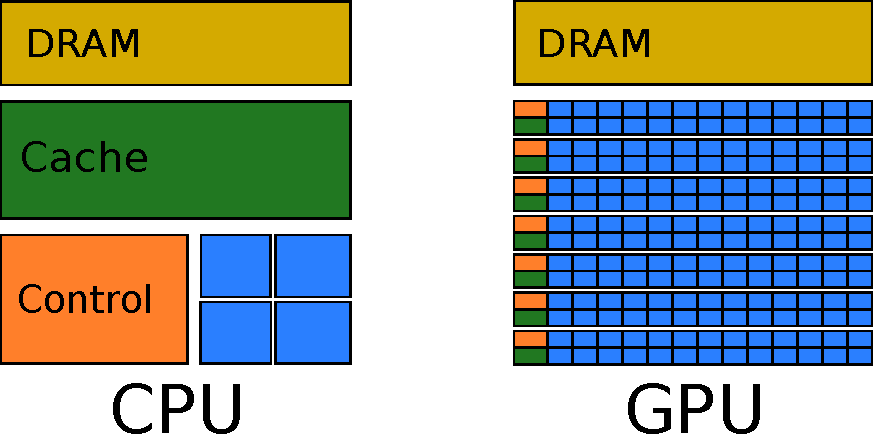
\includegraphics[width=0.8\textwidth]{img/architecture.pdf}
        \caption{CPU and GPU simplistic architecture model}
    \end{figure}
\end{frame}

\begin{frame}
    \frametitle{GPU Computing}
    \framesubtitle{Differences between CPU and GPU}
    \begin{itemize}
        \item Goals and design
        \begin{itemize}
            \item The CPU was designed to have a good performances with parallel and non-parallel
                  scenarios.
            \item The GPU was designed to do highly parallel work.
        \end{itemize}
        \item The CPU minimize \blue{latency} experienced by 1 thread (big on-chip caches).
        \item The GPU maximize \blue{throughput} of all threads.
    \end{itemize}
\end{frame}

\begin{frame}
    \frametitle{GPU Computing}
    \framesubtitle{}
    \begin{itemize}
        \item The GPU Computing \red{is not} the solution for every computational problem.
        \item It is mandatory to enter in the ``APOD'' design cycle.
    \end{itemize}
\end{frame}

\begin{frame}
    \frametitle{GPU Computing}
    \framesubtitle{APOD design cycle}
    \begin{figure}
        \centering
        \label{fig:apod}
        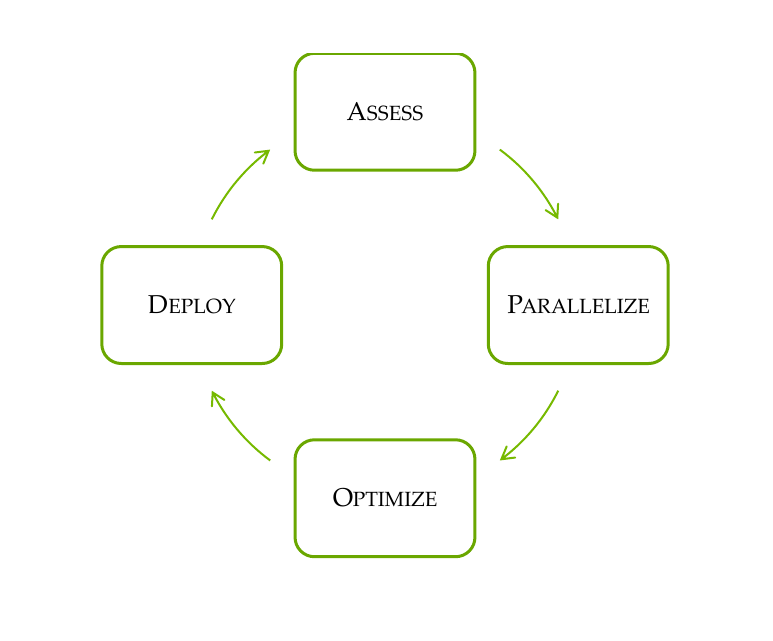
\includegraphics[width=0.7\textwidth]{img/apod}
        \caption{GPU Programming Cycle}
    \end{figure}
\end{frame}

\begin{frame}
    \frametitle{GPU Computing}
    \framesubtitle{APOD - Asses}
    \begin{itemize}
        \item What?
        \begin{itemize}
            \item Locate the code sections, responsible for the bulk of the execution time.
        \end{itemize}
        \item How?
        \begin{itemize}
            \item Using profiling tools (e.g. \texttt{gprof}, \texttt{vTune}, etc)
        \end{itemize}
    \end{itemize}
\end{frame}

\begin{frame}
    \frametitle{GPU Computing}
    \framesubtitle{APOD - Parallelize}
    \begin{itemize}
        \item What?
        \begin{itemize}
            \item Parallelize the ``hotspots''.
                (Be careful of the code refactoring!)
        \end{itemize}
        \item How?
        \begin{itemize}
            \item Using different techniques and libraries.
        \end{itemize}
    \end{itemize}
\end{frame}

\begin{frame}
    \frametitle{GPU Computing}
    \framesubtitle{APOD - Optimize}
    \begin{itemize}
        \item What?
        \begin{itemize}
            \item Optimize the current implementation (there are a lot of ways to do it!)
        \end{itemize}
        \item How?
        \begin{itemize}
            \item Doing a review of the following topics:
            \begin{itemize}
                \item Data transfer.
                \item Floating point operations (FLOPs).
                \item Loop unrolling.
                \item etc.
            \end{itemize}
        \end{itemize}
    \end{itemize}
\end{frame}

\begin{frame}
    \frametitle{GPU Computing}
    \framesubtitle{APOD - Deploy}
    \begin{itemize}
        \item What?
        \begin{itemize}
            \item Check if the current parallelization idea is enough for the program,
              before trying to improve another hotspot.
        \end{itemize}
        \item How?
        \begin{itemize}
            \item Comparing theoretical and experimental result of the current code.
        \end{itemize}
    \end{itemize}
\end{frame}
